\newpage
\section{Цель работы}
\hspace*{\parindent}Получить опыт определения математической модели исследуемого объекта управления.
Собрать требуемый роботехнический механизм.

\section{Порядок выполнения работы}
\hspace*{\parindent}Порядок выполнения данной лабораторной работы аналогичен тому, который был представлен в работе~№4.
Отдельно стоит отметить только две вещи.
Во-первых, для определения значений величин $\psi$ и $\dot\psi$ Segway следует оборудовать датчиком NXT Gyro Sensor (см.~Приложение А).
Во-вторых, при расчете момента инерции <<тела>> робота входящие в него командный блок, выше указанный датчик и сервоприводы следует принять за однородные параллелепипеды (рис.~\ref{paraps}).

\begin{figure}[h]
	\noindent\centering{ 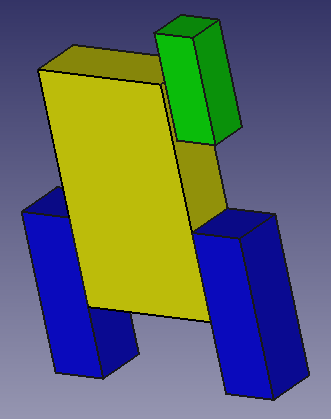
\includegraphics[scale=0.65]{paraps.png} }
	\caption{Аппроксимация Segway параллелепипедами.}
	\label{paraps}
\end{figure}

Момент инерции такого тела, относительно горизонтальной оси, проходящей через его центр масс и перпендикулярной направлению его движение, есть сумма моментов инерции относительно нее каждого из параллелепипедов. 
Напоминаем, что последние можно определить с помощью теоремы Штейнера. 

\newpage
\section{Приложение А\\
Основы работы с датчиком NXT Gyro Sensor}
\hspace*{\parindent}NXT Gyro Sensor представляет из себя модуль, изображенный на рис.~\ref{sensor}. 
Этот датчик возвращает значение собственной угловой скорости вращения относительно оси, перпендикулярной той его поверхности, которая обращена <<к нам>> на рис.~\ref{sensor}б.
Данный факт пояснен красной стрелкой, показанной там же.

\begin{figure}[h]
	\begin{minipage}[h]{0.49\linewidth}
		\center{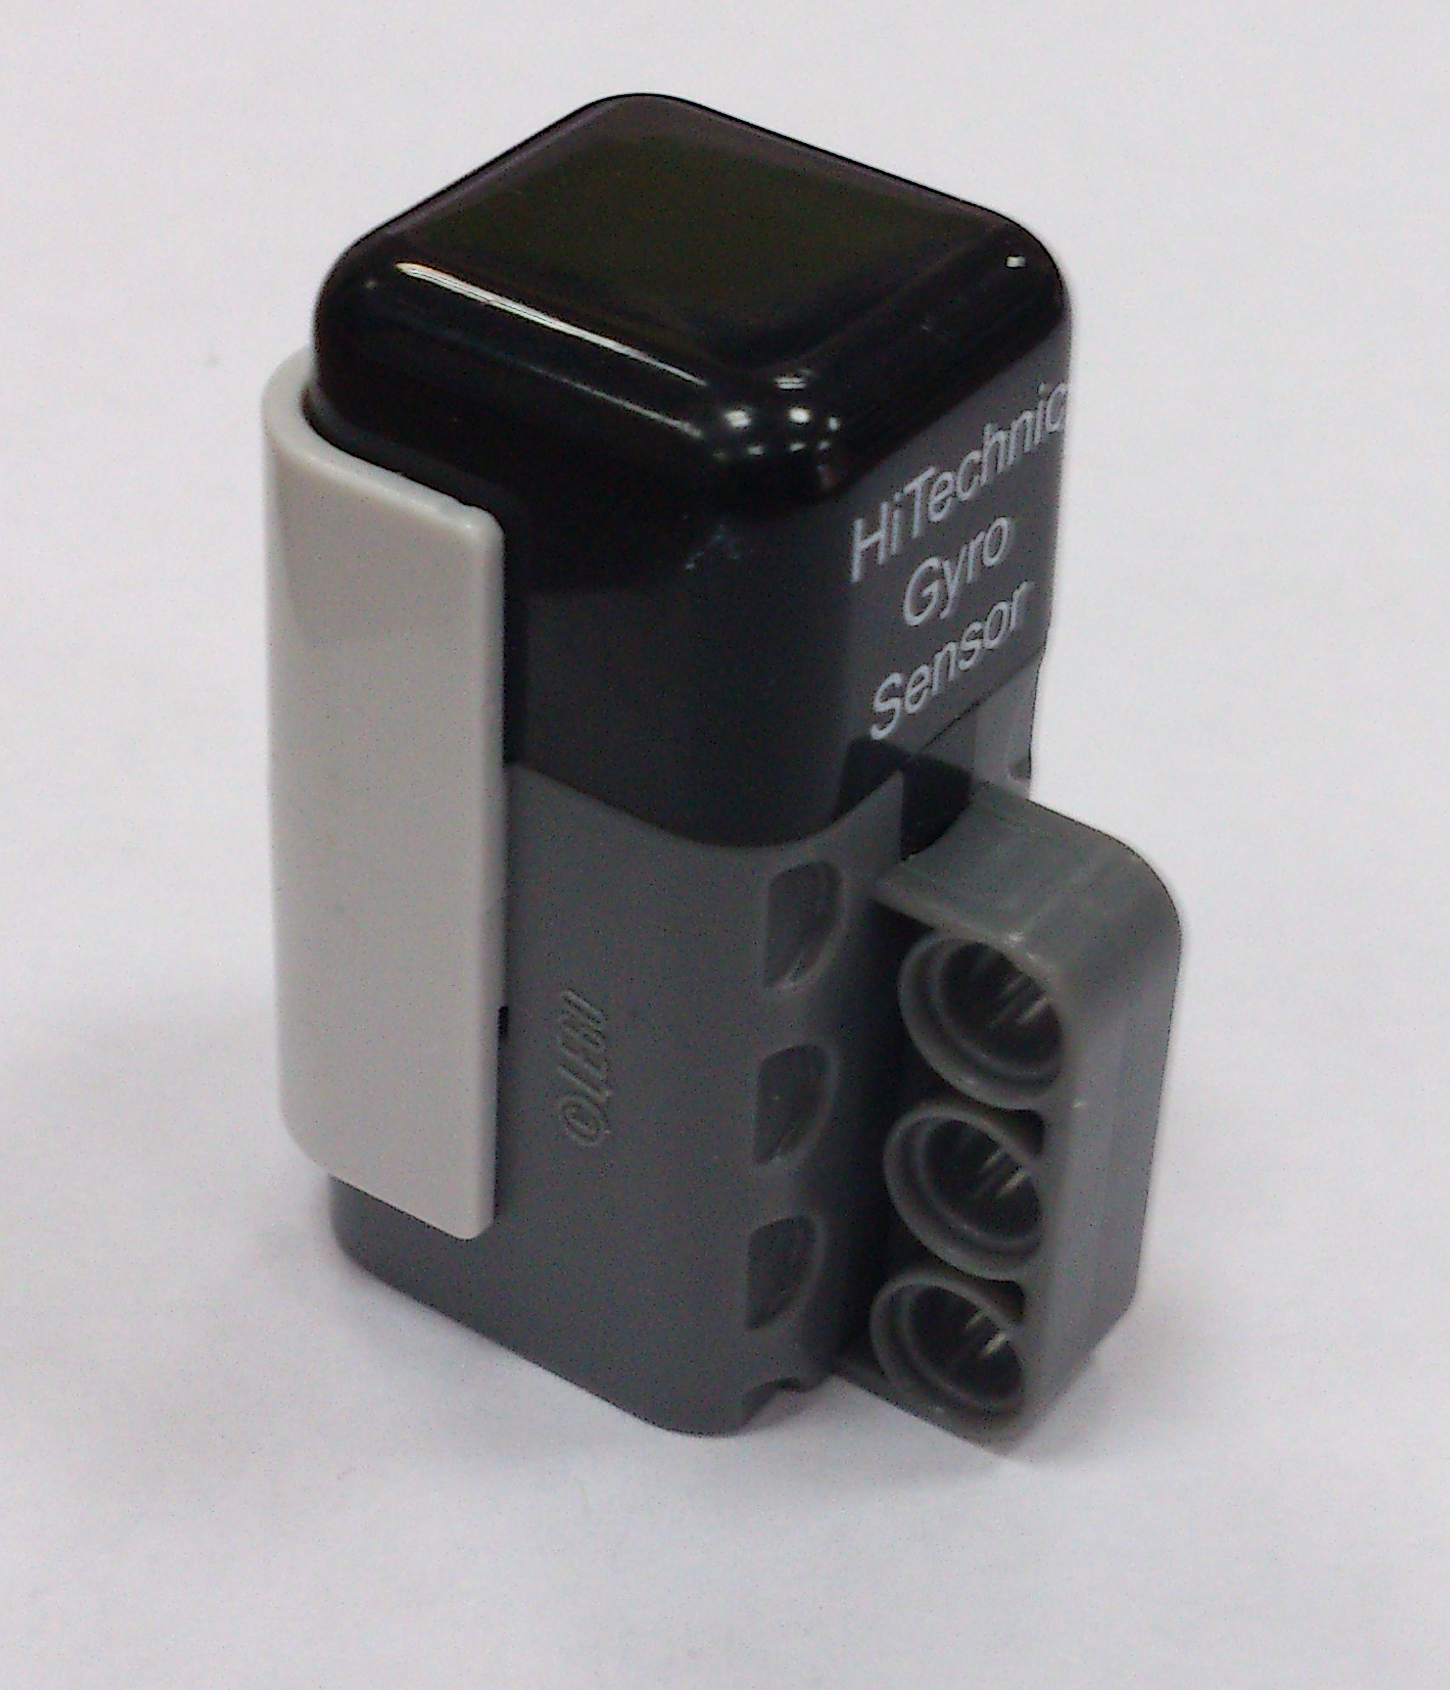
\includegraphics[height = 5.5 cm]{sensor_main.png} \\ а)}
	\end{minipage}
	\hfill
	\begin{minipage}[h]{0.49\linewidth}
		\center{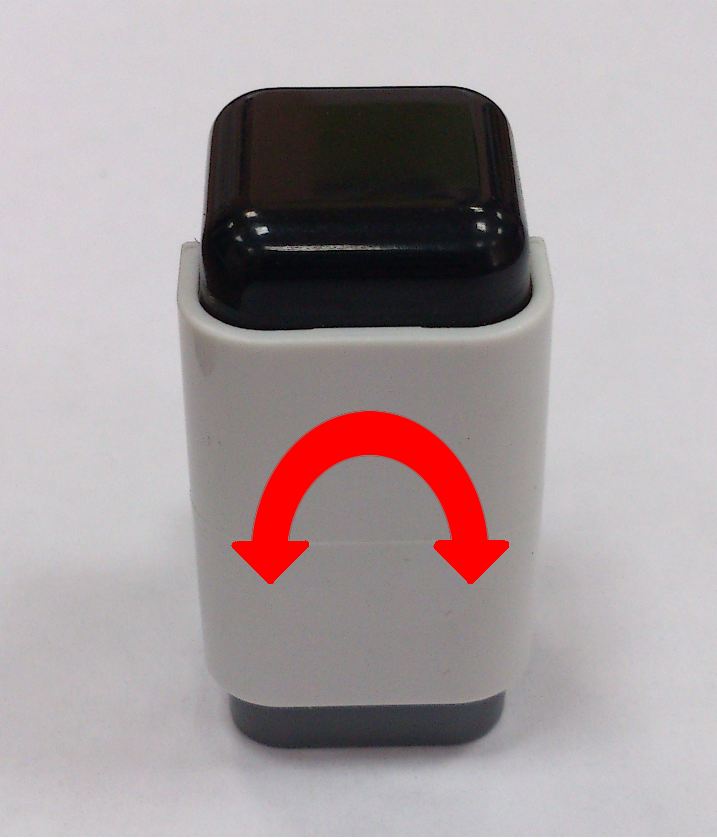
\includegraphics[height = 5.5 cm]{sensor_add.png} \\ б)}
	\end{minipage}
	\caption{Внешний вид NXT Gyro Sensor.}
	\label{sensor}
\end{figure}

Чтобы зарегистрировать NXT Gyro Sensor в исполняемой программе, в ее состав необходимо добавить функцию \verb|SetSensorHTGyro(sensor_port)|, чей единственный аргумент, как несложно догадаться, есть номер порта, в который этот датчик подключен.

Считывание данных производится функцией \verb|SensorHTGyro(sensor_port)|.
Возвращаемое ею целое значение представляет собой уже упомянутую угловую скорость, выраженную в [градусах в секунду].   
Знак получаемого числа определяется направлением вращения.

Особое внимание при работе с этим датчиком следует уделить тому, что в его данных может содержаться определенная ошибка, поэтому прежде, чем использовать сенсор в составе рабочего устройства, его необходимо дополнительно проверить. 
В случае, если указанная погрешность присутствует и носит простейший характер\lefteqn,\footnote{Например, датчик постоянно возвращает значение скорости на $n$ (градусов/с) меньшее или большее настоящего.} очевидно, что ее следует учесть, внеся определенные изменения в текст исполняемой роботом программы.